\documentclass[]{book}
\usepackage{lmodern}
\usepackage{amssymb,amsmath}
\usepackage{ifxetex,ifluatex}
\usepackage{fixltx2e} % provides \textsubscript
\ifnum 0\ifxetex 1\fi\ifluatex 1\fi=0 % if pdftex
  \usepackage[T1]{fontenc}
  \usepackage[utf8]{inputenc}
\else % if luatex or xelatex
  \ifxetex
    \usepackage{mathspec}
  \else
    \usepackage{fontspec}
  \fi
  \defaultfontfeatures{Ligatures=TeX,Scale=MatchLowercase}
\fi
% use upquote if available, for straight quotes in verbatim environments
\IfFileExists{upquote.sty}{\usepackage{upquote}}{}
% use microtype if available
\IfFileExists{microtype.sty}{%
\usepackage{microtype}
\UseMicrotypeSet[protrusion]{basicmath} % disable protrusion for tt fonts
}{}
\usepackage[margin=1in]{geometry}
\usepackage{hyperref}
\hypersetup{unicode=true,
            pdftitle={SMRT},
            pdfauthor={Chris Foster},
            pdfborder={0 0 0},
            breaklinks=true}
\urlstyle{same}  % don't use monospace font for urls
\usepackage{natbib}
\bibliographystyle{apalike}
\usepackage{color}
\usepackage{fancyvrb}
\newcommand{\VerbBar}{|}
\newcommand{\VERB}{\Verb[commandchars=\\\{\}]}
\DefineVerbatimEnvironment{Highlighting}{Verbatim}{commandchars=\\\{\}}
% Add ',fontsize=\small' for more characters per line
\usepackage{framed}
\definecolor{shadecolor}{RGB}{248,248,248}
\newenvironment{Shaded}{\begin{snugshade}}{\end{snugshade}}
\newcommand{\KeywordTok}[1]{\textcolor[rgb]{0.13,0.29,0.53}{\textbf{#1}}}
\newcommand{\DataTypeTok}[1]{\textcolor[rgb]{0.13,0.29,0.53}{#1}}
\newcommand{\DecValTok}[1]{\textcolor[rgb]{0.00,0.00,0.81}{#1}}
\newcommand{\BaseNTok}[1]{\textcolor[rgb]{0.00,0.00,0.81}{#1}}
\newcommand{\FloatTok}[1]{\textcolor[rgb]{0.00,0.00,0.81}{#1}}
\newcommand{\ConstantTok}[1]{\textcolor[rgb]{0.00,0.00,0.00}{#1}}
\newcommand{\CharTok}[1]{\textcolor[rgb]{0.31,0.60,0.02}{#1}}
\newcommand{\SpecialCharTok}[1]{\textcolor[rgb]{0.00,0.00,0.00}{#1}}
\newcommand{\StringTok}[1]{\textcolor[rgb]{0.31,0.60,0.02}{#1}}
\newcommand{\VerbatimStringTok}[1]{\textcolor[rgb]{0.31,0.60,0.02}{#1}}
\newcommand{\SpecialStringTok}[1]{\textcolor[rgb]{0.31,0.60,0.02}{#1}}
\newcommand{\ImportTok}[1]{#1}
\newcommand{\CommentTok}[1]{\textcolor[rgb]{0.56,0.35,0.01}{\textit{#1}}}
\newcommand{\DocumentationTok}[1]{\textcolor[rgb]{0.56,0.35,0.01}{\textbf{\textit{#1}}}}
\newcommand{\AnnotationTok}[1]{\textcolor[rgb]{0.56,0.35,0.01}{\textbf{\textit{#1}}}}
\newcommand{\CommentVarTok}[1]{\textcolor[rgb]{0.56,0.35,0.01}{\textbf{\textit{#1}}}}
\newcommand{\OtherTok}[1]{\textcolor[rgb]{0.56,0.35,0.01}{#1}}
\newcommand{\FunctionTok}[1]{\textcolor[rgb]{0.00,0.00,0.00}{#1}}
\newcommand{\VariableTok}[1]{\textcolor[rgb]{0.00,0.00,0.00}{#1}}
\newcommand{\ControlFlowTok}[1]{\textcolor[rgb]{0.13,0.29,0.53}{\textbf{#1}}}
\newcommand{\OperatorTok}[1]{\textcolor[rgb]{0.81,0.36,0.00}{\textbf{#1}}}
\newcommand{\BuiltInTok}[1]{#1}
\newcommand{\ExtensionTok}[1]{#1}
\newcommand{\PreprocessorTok}[1]{\textcolor[rgb]{0.56,0.35,0.01}{\textit{#1}}}
\newcommand{\AttributeTok}[1]{\textcolor[rgb]{0.77,0.63,0.00}{#1}}
\newcommand{\RegionMarkerTok}[1]{#1}
\newcommand{\InformationTok}[1]{\textcolor[rgb]{0.56,0.35,0.01}{\textbf{\textit{#1}}}}
\newcommand{\WarningTok}[1]{\textcolor[rgb]{0.56,0.35,0.01}{\textbf{\textit{#1}}}}
\newcommand{\AlertTok}[1]{\textcolor[rgb]{0.94,0.16,0.16}{#1}}
\newcommand{\ErrorTok}[1]{\textcolor[rgb]{0.64,0.00,0.00}{\textbf{#1}}}
\newcommand{\NormalTok}[1]{#1}
\usepackage{longtable,booktabs}
\usepackage{graphicx,grffile}
\makeatletter
\def\maxwidth{\ifdim\Gin@nat@width>\linewidth\linewidth\else\Gin@nat@width\fi}
\def\maxheight{\ifdim\Gin@nat@height>\textheight\textheight\else\Gin@nat@height\fi}
\makeatother
% Scale images if necessary, so that they will not overflow the page
% margins by default, and it is still possible to overwrite the defaults
% using explicit options in \includegraphics[width, height, ...]{}
\setkeys{Gin}{width=\maxwidth,height=\maxheight,keepaspectratio}
\IfFileExists{parskip.sty}{%
\usepackage{parskip}
}{% else
\setlength{\parindent}{0pt}
\setlength{\parskip}{6pt plus 2pt minus 1pt}
}
\setlength{\emergencystretch}{3em}  % prevent overfull lines
\providecommand{\tightlist}{%
  \setlength{\itemsep}{0pt}\setlength{\parskip}{0pt}}
\setcounter{secnumdepth}{5}
% Redefines (sub)paragraphs to behave more like sections
\ifx\paragraph\undefined\else
\let\oldparagraph\paragraph
\renewcommand{\paragraph}[1]{\oldparagraph{#1}\mbox{}}
\fi
\ifx\subparagraph\undefined\else
\let\oldsubparagraph\subparagraph
\renewcommand{\subparagraph}[1]{\oldsubparagraph{#1}\mbox{}}
\fi

%%% Use protect on footnotes to avoid problems with footnotes in titles
\let\rmarkdownfootnote\footnote%
\def\footnote{\protect\rmarkdownfootnote}

%%% Change title format to be more compact
\usepackage{titling}

% Create subtitle command for use in maketitle
\newcommand{\subtitle}[1]{
  \posttitle{
    \begin{center}\large#1\end{center}
    }
}

\setlength{\droptitle}{-2em}

  \title{SMRT}
    \pretitle{\vspace{\droptitle}\centering\huge}
  \posttitle{\par}
    \author{Chris Foster}
    \preauthor{\centering\large\emph}
  \postauthor{\par}
      \predate{\centering\large\emph}
  \postdate{\par}
    \date{2018-09-14}

\usepackage{booktabs}

\usepackage{amsthm}
\newtheorem{theorem}{Theorem}[chapter]
\newtheorem{lemma}{Lemma}[chapter]
\theoremstyle{definition}
\newtheorem{definition}{Definition}[chapter]
\newtheorem{corollary}{Corollary}[chapter]
\newtheorem{proposition}{Proposition}[chapter]
\theoremstyle{definition}
\newtheorem{example}{Example}[chapter]
\theoremstyle{definition}
\newtheorem{exercise}{Exercise}[chapter]
\theoremstyle{remark}
\newtheorem*{remark}{Remark}
\newtheorem*{solution}{Solution}
\begin{document}
\maketitle

{
\setcounter{tocdepth}{1}
\tableofcontents
}
\chapter{Preface}\label{preface}

This book is a \textbf{compilation} of different reseach pieces all
compiled together into a single volume. The purpose of the volume is to
provide a concise, research oriented view of the smart item and other
accompanying item formats. Each chapter will be a different research
topic and we will attempt to group similar research articles in close
proximity to each other within the book.

\chapter{Introduction to Smart Items}\label{introduction-to-smart-items}

A SmartItem is first and foremost an item, used on exams to measure
important skills. Like traditional items, it has an ID number, is stored
on a computer, is evaluated like traditional items with expert reviews,
and eventually response data from examinees. It can be used on any kind
of test design, such as CAT, LOFT, etc. If and when it doesn't function
well, it can be repaired or deleted or retired.

The main difference between a smart item and a normal item is that the
smart item is written with three areas of expertise: Subject matter,
item writing and programming. With a well written and specific
objective, with the help of a programmer and enough content expertise it
is possible to write a single item which can cover the entire range of
an objective. With the help of a programmer an item writer can write a
series of stems, options, correct responses and incorrect responses that
can generate a large amount of potential item derivatives based on a
single objective. This process creates an item that is less static than
a single multiple choice item.

In order better understand a smart item it is best to start with an
example. An illustrativec example would come from an elementary math
test. A single objective might be: Add two single digit numbers. There
are only 10 single digit numbers (including 0) So really there is only
(10!/ 2!(10-2)!) = 45 possible options as long as order doesn't matter.

Now, a single item writer could write all 45 items and cover the
objective completely. However, it is also possible to write a simple
program which generates all 45 possible questions. Now, for a fixed form
test it would be likely that the item writer woudl not write all 45
options but instead write 2 or 3 of which one would be selected for the
first form of the test while a different one might be selected for a
second form. However, when administering a smart item to participants
each participant would get a random stem and random options (including
the correct option).

Now, for a simple math objective it might not be necessary to write an
algorithm that writes the 45 different possible stems for the objective.
However, imagine an objective where there are 206 possible answers such
as ``Identify each bone in the human body.'' Or perhaps there is an
objective which asks participants to arrange 4 words in alphabetical
order. The words can be anything in the human dictionary. Now there are
170,000 words in the english language and picking 4 leaves
3.479x10\^{}19 possible options to completely cover the objective
content and no item writer can write all of them and given current test
construction methods there is no reason to do so.

\section{Purpose of Building Smart
Items}\label{purpose-of-building-smart-items}

\section{Smart Item Logic}\label{smart-item-logic}

A first step to understanding the logic behind smart items is to
understand the logic of randomization in experimentation. In 1925 Sir
Ronald Fisher \citet{fisher1925} outlined what is considered the
cornerstone of experimental research today: randomization. Randomization
has three primary purposes:

\begin{enumerate}
\def\labelenumi{\arabic{enumi})}
\item
  It helps to distribute idosyncratic characteristics of participants to
  groups so that it does not bias the outcome. If participants could
  self select groups or were grouped based on characteristics than it
  could create systematic biases in the outcome based on participant
  characteristics.
\item
  Randomization helps calculate unbiased estimate of error effects. IE:
  those effects not attributable to the manipulation of an independent
  variable
\item
  Randomization helps ensure that error efects are statistically
  independent.
\end{enumerate}

Now, considering point \#1 a bit more: Randomization helps ensure that
within group variability is Independent and identically distributed
(IID) or in other words, within group variability does not contain bias
and is simply noise. Without randomization it could easily contain any
number of biases which could decrease or increase the differnces between
groups. It is impossible to list all possible systematic biases that
could creep into an experiment. Maybe all college educated participants
self select themselves into a specific group or one gender reacts
differently to a group assignment than another.

While other papers have talked in length about the importance of
randomization in experimental design for the purposes of this section
randomization removes systematic bias within group.

One natural artifact of the randomization process is an increase in
within-group variation. If participants are asigned to groups based on
characterisitcs or allowed to self select, more similar participants
will end up in the same group reducing the amount of variability in the
group. While a decrease in within-group variability inevitibly increases
the probability of a significant effect in an experiment, the
significant effect may simply be due to a bias brought by the selection
process\ldots{} which simply shows the importance of randomization. Even
though variation is introduced, results are more trustworthy.

\chapter{DOMC Difficulty Variance}\label{domc-difficulty-variance}

\section{Initial Run}\label{initial-run}

Here is a document showing the results of item families derived from a
single DOMC stem. Essentially we treat each possible combination of
options as a different question just to see the amount of variance from
a single DOMC stem.

In this first run we treat each different option combination as a
different item, including those for people who never saw the correct
response (making all these p-values 0)

\begin{Shaded}
\begin{Highlighting}[]
\KeywordTok{library}\NormalTok{(dplyr)}
\KeywordTok{library}\NormalTok{(readr)}
\KeywordTok{library}\NormalTok{(knitr)}
\KeywordTok{library}\NormalTok{(ggplot2)}
\KeywordTok{library}\NormalTok{(lemon)}

\NormalTok{setwd_thisdir <-}\StringTok{ }\ControlFlowTok{function}\NormalTok{ () \{}
\NormalTok{  this.dir <-}\StringTok{ }\KeywordTok{dirname}\NormalTok{(}\KeywordTok{parent.frame}\NormalTok{(}\DecValTok{3}\NormalTok{)}\OperatorTok{$}\NormalTok{ofile)}
  \KeywordTok{setwd}\NormalTok{(this.dir)}
\NormalTok{\}}


\NormalTok{hp_data =}\StringTok{ }\KeywordTok{read_csv}\NormalTok{(}\StringTok{'data/domc_order_difficulty/Full Responses After Exclusions.csv'}\NormalTok{)}

\NormalTok{hp_clean =}\StringTok{ }\NormalTok{hp_data }\OperatorTok\StringTok{ }\KeywordTok{filter}\NormalTok{(item_type }\OperatorTok{==}\StringTok{ 'domc'}\NormalTok{, item_component_type }\OperatorTok{==}\StringTok{ 'domc_option'}\NormalTok{) }\OperatorTok\StringTok{ }\KeywordTok{group_by}\NormalTok{(delivery_id, item_id) }\OperatorTok\StringTok{ }\KeywordTok{mutate}\NormalTok{(}\DataTypeTok{option_order =} \KeywordTok{paste0}\NormalTok{(option_presented, }\DataTypeTok{collapse =} \StringTok{""}\NormalTok{))}

\NormalTok{hp_summary =}\StringTok{ }\NormalTok{hp_clean }\OperatorTok\StringTok{ }\KeywordTok{group_by}\NormalTok{(delivery_id, item_id) }\OperatorTok\StringTok{ }\KeywordTok{summarize}\NormalTok{(}\DataTypeTok{item_total_seconds =} \KeywordTok{max}\NormalTok{(item_total_seconds), }\DataTypeTok{item_order =} \KeywordTok{max}\NormalTok{(option_order), }\DataTypeTok{score =} \KeywordTok{max}\NormalTok{(score)) }\OperatorTok\StringTok{ }\KeywordTok{group_by}\NormalTok{(delivery_id, item_id) }\OperatorTok\StringTok{ }\KeywordTok{mutate}\NormalTok{(}\DataTypeTok{order =} \KeywordTok{paste}\NormalTok{(}\KeywordTok{sort}\NormalTok{(}\KeywordTok{unlist}\NormalTok{(}\KeywordTok{strsplit}\NormalTok{(}\KeywordTok{as.character}\NormalTok{(item_order), }\StringTok{""}\NormalTok{))), }\DataTypeTok{collapse =} \StringTok{""}\NormalTok{)) }

\NormalTok{hp_items =}\StringTok{ }\NormalTok{hp_summary }\OperatorTok\StringTok{ }\KeywordTok{group_by}\NormalTok{(item_id, order) }\OperatorTok\StringTok{ }\KeywordTok{summarize}\NormalTok{(}\DataTypeTok{p_value =} \KeywordTok{mean}\NormalTok{(score), }\DataTypeTok{count =} \KeywordTok{n}\NormalTok{())}
\end{Highlighting}
\end{Shaded}

\section{Item 10B\_v1}\label{item-10b_v1}

\begin{Shaded}
\begin{Highlighting}[]
\NormalTok{tenb_v1 =}\StringTok{ }\NormalTok{hp_items }\OperatorTok\StringTok{ }\KeywordTok{filter}\NormalTok{(item_id }\OperatorTok{==}\StringTok{ '10B_v1'}\NormalTok{)}
\KeywordTok{kable}\NormalTok{(tenb_v1)}
\end{Highlighting}
\end{Shaded}

\begin{tabular}{l|l|r|r}
\hline
item\_id & order & p\_value & count\\
\hline
10B\_v1 & 0 & 0.8950000 & 200\\
\hline
10B\_v1 & 01 & 1.0000000 & 42\\
\hline
10B\_v1 & 012 & 0.9677419 & 31\\
\hline
10B\_v1 & 0123 & 1.0000000 & 40\\
\hline
10B\_v1 & 01234 & 0.9876543 & 162\\
\hline
10B\_v1 & 0124 & 0.9827586 & 58\\
\hline
10B\_v1 & 013 & 0.9666667 & 30\\
\hline
10B\_v1 & 0134 & 1.0000000 & 45\\
\hline
10B\_v1 & 014 & 0.9629630 & 27\\
\hline
10B\_v1 & 02 & 0.9365079 & 63\\
\hline
10B\_v1 & 023 & 0.9487179 & 39\\
\hline
10B\_v1 & 0234 & 0.9354839 & 62\\
\hline
10B\_v1 & 024 & 0.9210526 & 38\\
\hline
10B\_v1 & 03 & 0.9464286 & 56\\
\hline
10B\_v1 & 034 & 0.9666667 & 30\\
\hline
10B\_v1 & 04 & 0.9756098 & 41\\
\hline
10B\_v1 & 1 & 0.0000000 & 21\\
\hline
10B\_v1 & 12 & 0.0000000 & 6\\
\hline
10B\_v1 & 123 & 0.0000000 & 8\\
\hline
10B\_v1 & 1234 & 0.0000000 & 13\\
\hline
10B\_v1 & 124 & 0.0000000 & 3\\
\hline
10B\_v1 & 13 & 0.0000000 & 10\\
\hline
10B\_v1 & 134 & 0.0000000 & 7\\
\hline
10B\_v1 & 14 & 0.0000000 & 8\\
\hline
10B\_v1 & 2 & 0.0000000 & 3\\
\hline
10B\_v1 & 234 & 0.0000000 & 1\\
\hline
10B\_v1 & 24 & 0.0000000 & 4\\
\hline
10B\_v1 & 3 & 0.0000000 & 1\\
\hline
10B\_v1 & 4 & 0.0000000 & 2\\
\hline
\end{tabular}

\subsection{Histogram}\label{histogram}

\begin{Shaded}
\begin{Highlighting}[]
\KeywordTok{theme_update}\NormalTok{(}\DataTypeTok{plot.title =} \KeywordTok{element_text}\NormalTok{(}\DataTypeTok{hjust =} \FloatTok{0.5}\NormalTok{))}
\KeywordTok{ggplot}\NormalTok{(tenb_v1, }\KeywordTok{aes}\NormalTok{(}\DataTypeTok{x=}\NormalTok{p_value)) }\OperatorTok{+}\StringTok{ }\KeywordTok{geom_histogram}\NormalTok{(}\DataTypeTok{binwidth=}\NormalTok{.}\DecValTok{01}\NormalTok{) }\OperatorTok{+}\StringTok{ }\KeywordTok{labs}\NormalTok{(}\DataTypeTok{title =} \StringTok{"Item10B_v1"}\NormalTok{) }
\end{Highlighting}
\end{Shaded}

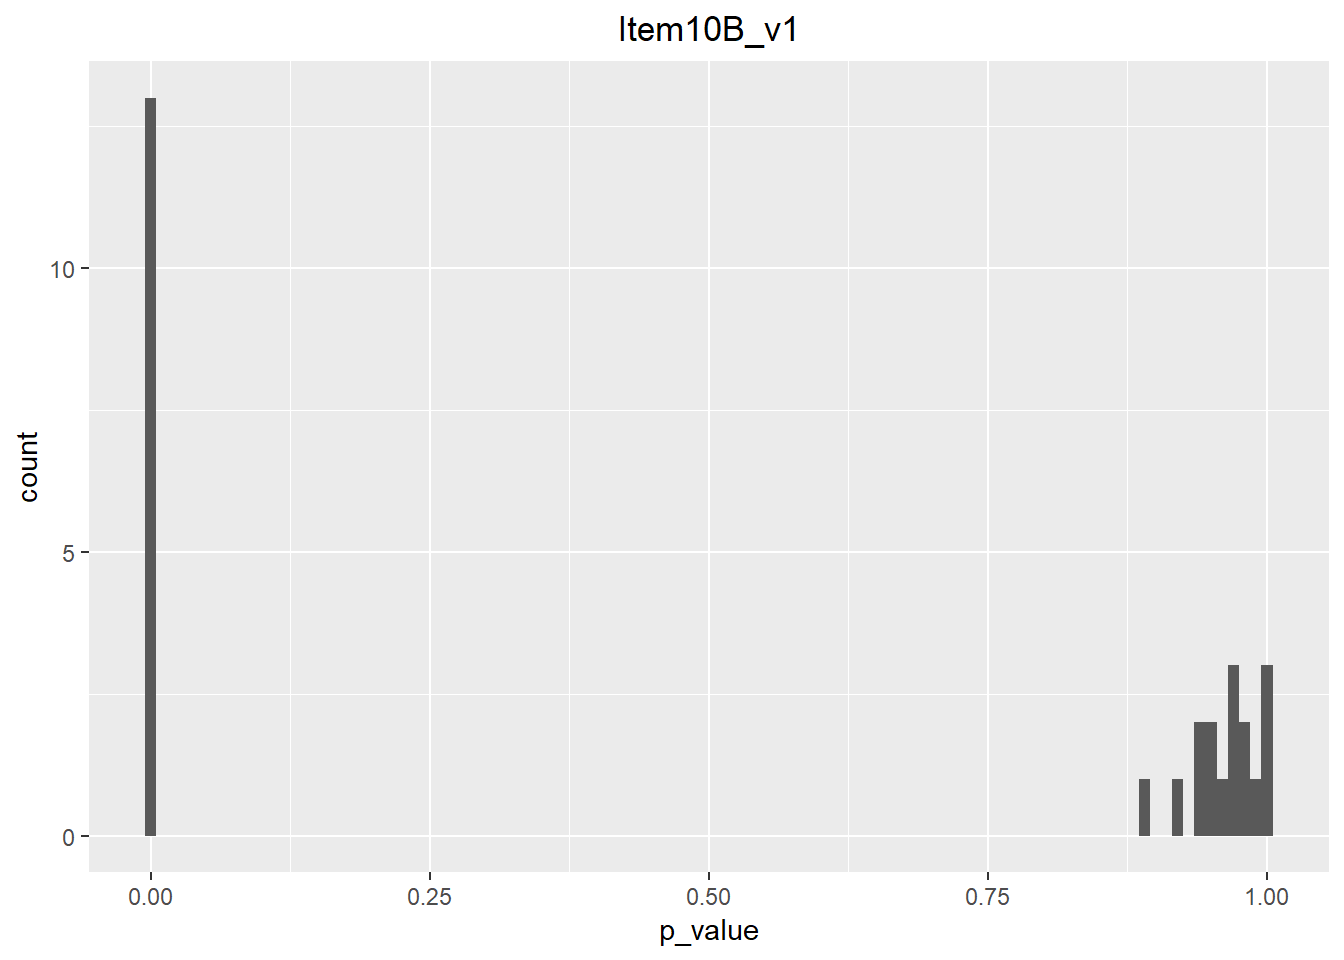
\includegraphics{smartitem_files/figure-latex/unnamed-chunk-4-1.pdf}

\section{Item 14b\_v1}\label{item-14b_v1}

\begin{Shaded}
\begin{Highlighting}[]
\NormalTok{fourteenb_v1 =}\StringTok{ }\NormalTok{hp_items }\OperatorTok\StringTok{ }\KeywordTok{filter}\NormalTok{(item_id }\OperatorTok{==}\StringTok{ '14B_v1'}\NormalTok{)}
\KeywordTok{kable}\NormalTok{(fourteenb_v1, }\DataTypeTok{format =} \StringTok{"markdown"}\NormalTok{)}
\end{Highlighting}
\end{Shaded}

\begin{longtable}[]{@{}llrr@{}}
\toprule
item\_id & order & p\_value & count\tabularnewline
\midrule
\endhead
14B\_v1 & 0 & 0.4235294 & 170\tabularnewline
14B\_v1 & 01 & 0.2765957 & 47\tabularnewline
14B\_v1 & 012 & 0.3636364 & 11\tabularnewline
14B\_v1 & 0123 & 0.2941176 & 17\tabularnewline
14B\_v1 & 01234 & 0.7049180 & 61\tabularnewline
14B\_v1 & 0124 & 0.7500000 & 12\tabularnewline
14B\_v1 & 013 & 0.5652174 & 23\tabularnewline
14B\_v1 & 0134 & 0.5666667 & 30\tabularnewline
14B\_v1 & 014 & 0.4583333 & 24\tabularnewline
14B\_v1 & 02 & 0.5263158 & 19\tabularnewline
14B\_v1 & 023 & 0.7500000 & 16\tabularnewline
14B\_v1 & 0234 & 0.4545455 & 11\tabularnewline
14B\_v1 & 024 & 0.6470588 & 17\tabularnewline
14B\_v1 & 03 & 0.4181818 & 55\tabularnewline
14B\_v1 & 034 & 0.5555556 & 36\tabularnewline
14B\_v1 & 04 & 0.4333333 & 30\tabularnewline
14B\_v1 & 1 & 0.0000000 & 39\tabularnewline
14B\_v1 & 12 & 0.0000000 & 23\tabularnewline
14B\_v1 & 123 & 0.0000000 & 22\tabularnewline
14B\_v1 & 1234 & 0.0000000 & 36\tabularnewline
14B\_v1 & 124 & 0.0000000 & 19\tabularnewline
14B\_v1 & 13 & 0.0000000 & 8\tabularnewline
14B\_v1 & 134 & 0.0000000 & 11\tabularnewline
14B\_v1 & 14 & 0.0000000 & 9\tabularnewline
14B\_v1 & 2 & 0.0000000 & 129\tabularnewline
14B\_v1 & 23 & 0.0000000 & 35\tabularnewline
14B\_v1 & 234 & 0.0000000 & 21\tabularnewline
14B\_v1 & 24 & 0.0000000 & 20\tabularnewline
14B\_v1 & 3 & 0.0000000 & 30\tabularnewline
14B\_v1 & 34 & 0.0000000 & 11\tabularnewline
14B\_v1 & 4 & 0.0000000 & 59\tabularnewline
\bottomrule
\end{longtable}

\subsection{Histogram}\label{histogram-1}

\begin{Shaded}
\begin{Highlighting}[]
\KeywordTok{ggplot}\NormalTok{(fourteenb_v1, }\KeywordTok{aes}\NormalTok{(}\DataTypeTok{x=}\NormalTok{p_value)) }\OperatorTok{+}\StringTok{ }\KeywordTok{geom_histogram}\NormalTok{(}\DataTypeTok{binwidth=}\NormalTok{.}\DecValTok{01}\NormalTok{) }\OperatorTok{+}\StringTok{ }\KeywordTok{labs}\NormalTok{(}\DataTypeTok{title =} \StringTok{"Item14B_v1"}\NormalTok{)}\OperatorTok{+}\StringTok{ }\KeywordTok{xlim}\NormalTok{(}\OperatorTok{-}\NormalTok{.}\DecValTok{01}\NormalTok{,}\DecValTok{1}\NormalTok{) }\OperatorTok{+}\StringTok{ }\KeywordTok{ylim}\NormalTok{(}\DecValTok{0}\NormalTok{,}\DecValTok{20}\NormalTok{)}
\end{Highlighting}
\end{Shaded}

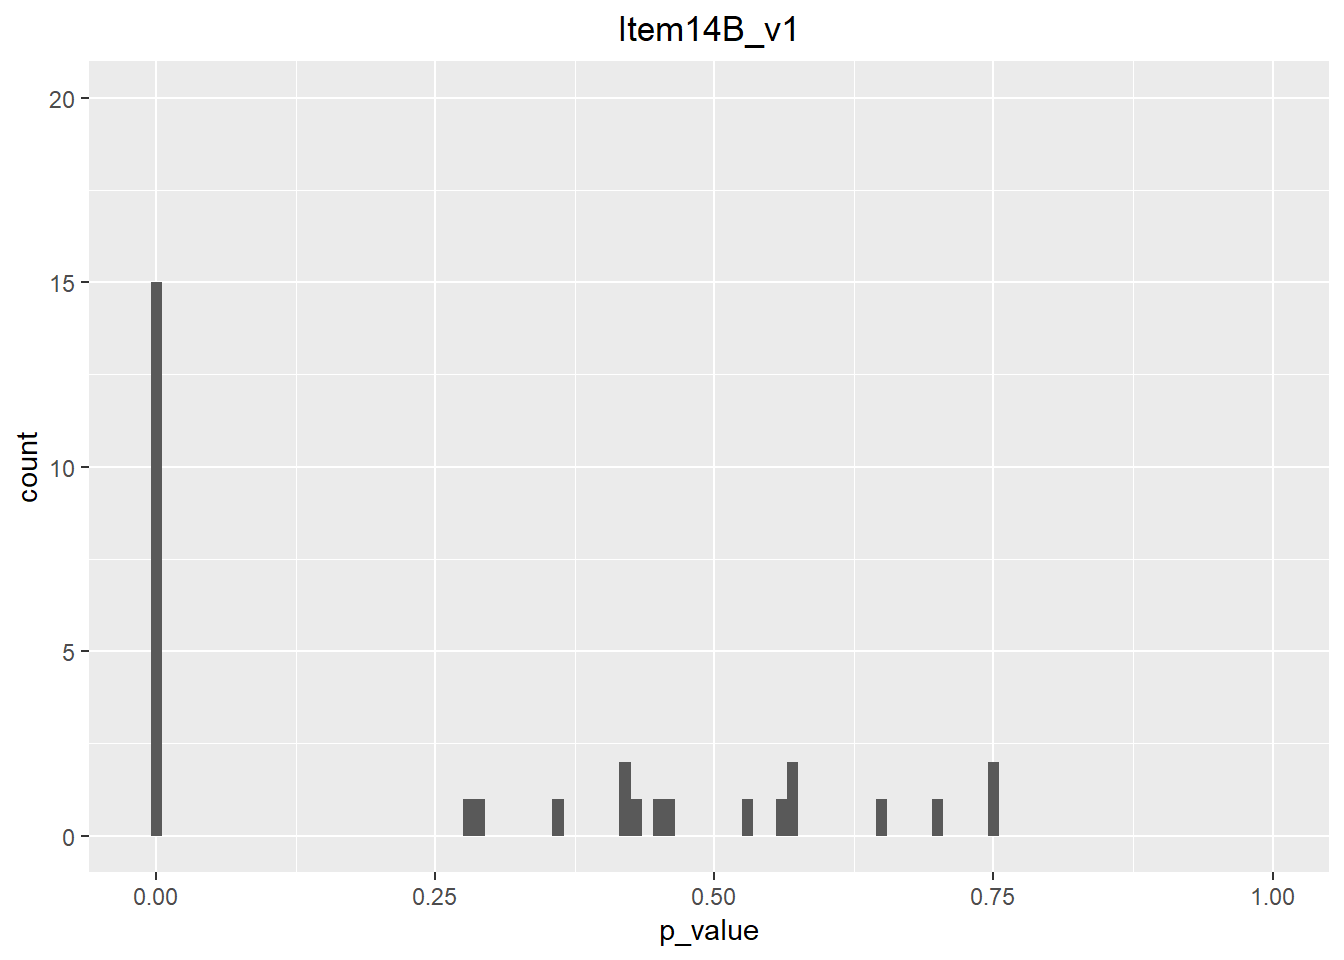
\includegraphics{smartitem_files/figure-latex/unnamed-chunk-6-1.pdf}

\section{Remove correct response}\label{remove-correct-response}

We notice quickly that it is pretty difficult to interpret the p-values
given that there is a significant amount of peole who never see the
correct answer so the p-value for those ``children'' is 0. Here is what
happens when we redefine what it means to be a different item. Instead
of looking at every combination of seen options we are only going to
look at distractors. This means that someone who saw the correct option
and the first option (coded 01) will have ``seen'' the ``same'' question
as someone who just saw the first distractor(coded 1).

It cleans things up a bit but it is important to recognize what is going
on.

\begin{Shaded}
\begin{Highlighting}[]
\NormalTok{hp_summary}\OperatorTok{$}\NormalTok{order_no_cr =}\StringTok{ }\KeywordTok{gsub}\NormalTok{(}\StringTok{'0'}\NormalTok{,}\StringTok{''}\NormalTok{,hp_summary}\OperatorTok{$}\NormalTok{order)}
\NormalTok{hp_summary}\OperatorTok{$}\NormalTok{order_no_cr =}\StringTok{ }\KeywordTok{ifelse}\NormalTok{(hp_summary}\OperatorTok{$}\NormalTok{order_no_cr }\OperatorTok{==}\StringTok{ ''}\NormalTok{, }\StringTok{'0'}\NormalTok{, hp_summary}\OperatorTok{$}\NormalTok{order_no_cr)}
\NormalTok{hp_items_no_cr =}\StringTok{ }\NormalTok{hp_summary }\OperatorTok\StringTok{ }\KeywordTok{group_by}\NormalTok{(item_id, order_no_cr) }\OperatorTok\StringTok{ }\KeywordTok{summarize}\NormalTok{(}\DataTypeTok{p_value =} \KeywordTok{mean}\NormalTok{(score), }\DataTypeTok{count =} \KeywordTok{n}\NormalTok{())}
\end{Highlighting}
\end{Shaded}

\section{Item 10B\_v1}\label{item-10b_v1-1}

\begin{Shaded}
\begin{Highlighting}[]
\NormalTok{tenb_v1 =}\StringTok{ }\NormalTok{hp_items_no_cr }\OperatorTok\StringTok{ }\KeywordTok{filter}\NormalTok{(item_id }\OperatorTok{==}\StringTok{ '10B_v1'}\NormalTok{)}
\KeywordTok{kable}\NormalTok{(tenb_v1)}
\end{Highlighting}
\end{Shaded}

\begin{tabular}{l|l|r|r}
\hline
item\_id & order\_no\_cr & p\_value & count\\
\hline
10B\_v1 & 0 & 0.8950000 & 200\\
\hline
10B\_v1 & 1 & 0.6666667 & 63\\
\hline
10B\_v1 & 12 & 0.8108108 & 37\\
\hline
10B\_v1 & 123 & 0.8333333 & 48\\
\hline
10B\_v1 & 1234 & 0.9142857 & 175\\
\hline
10B\_v1 & 124 & 0.9344262 & 61\\
\hline
10B\_v1 & 13 & 0.7250000 & 40\\
\hline
10B\_v1 & 134 & 0.8653846 & 52\\
\hline
10B\_v1 & 14 & 0.7428571 & 35\\
\hline
10B\_v1 & 2 & 0.8939394 & 66\\
\hline
10B\_v1 & 23 & 0.9487179 & 39\\
\hline
10B\_v1 & 234 & 0.9206349 & 63\\
\hline
10B\_v1 & 24 & 0.8333333 & 42\\
\hline
10B\_v1 & 3 & 0.9298246 & 57\\
\hline
10B\_v1 & 34 & 0.9666667 & 30\\
\hline
10B\_v1 & 4 & 0.9302326 & 43\\
\hline
\end{tabular}

\subsection{Histogram}\label{histogram-2}

\begin{Shaded}
\begin{Highlighting}[]
\KeywordTok{theme_update}\NormalTok{(}\DataTypeTok{plot.title =} \KeywordTok{element_text}\NormalTok{(}\DataTypeTok{hjust =} \FloatTok{0.5}\NormalTok{))}
\KeywordTok{ggplot}\NormalTok{(tenb_v1, }\KeywordTok{aes}\NormalTok{(}\DataTypeTok{x=}\NormalTok{p_value)) }\OperatorTok{+}\StringTok{ }\KeywordTok{geom_histogram}\NormalTok{(}\DataTypeTok{binwidth=}\NormalTok{.}\DecValTok{01}\NormalTok{) }\OperatorTok{+}\StringTok{ }\KeywordTok{labs}\NormalTok{(}\DataTypeTok{title =} \StringTok{"Item10B_v1"}\NormalTok{) }\OperatorTok{+}\StringTok{ }\KeywordTok{xlim}\NormalTok{(}\OperatorTok{-}\NormalTok{.}\DecValTok{01}\NormalTok{,}\DecValTok{1}\NormalTok{)}
\end{Highlighting}
\end{Shaded}

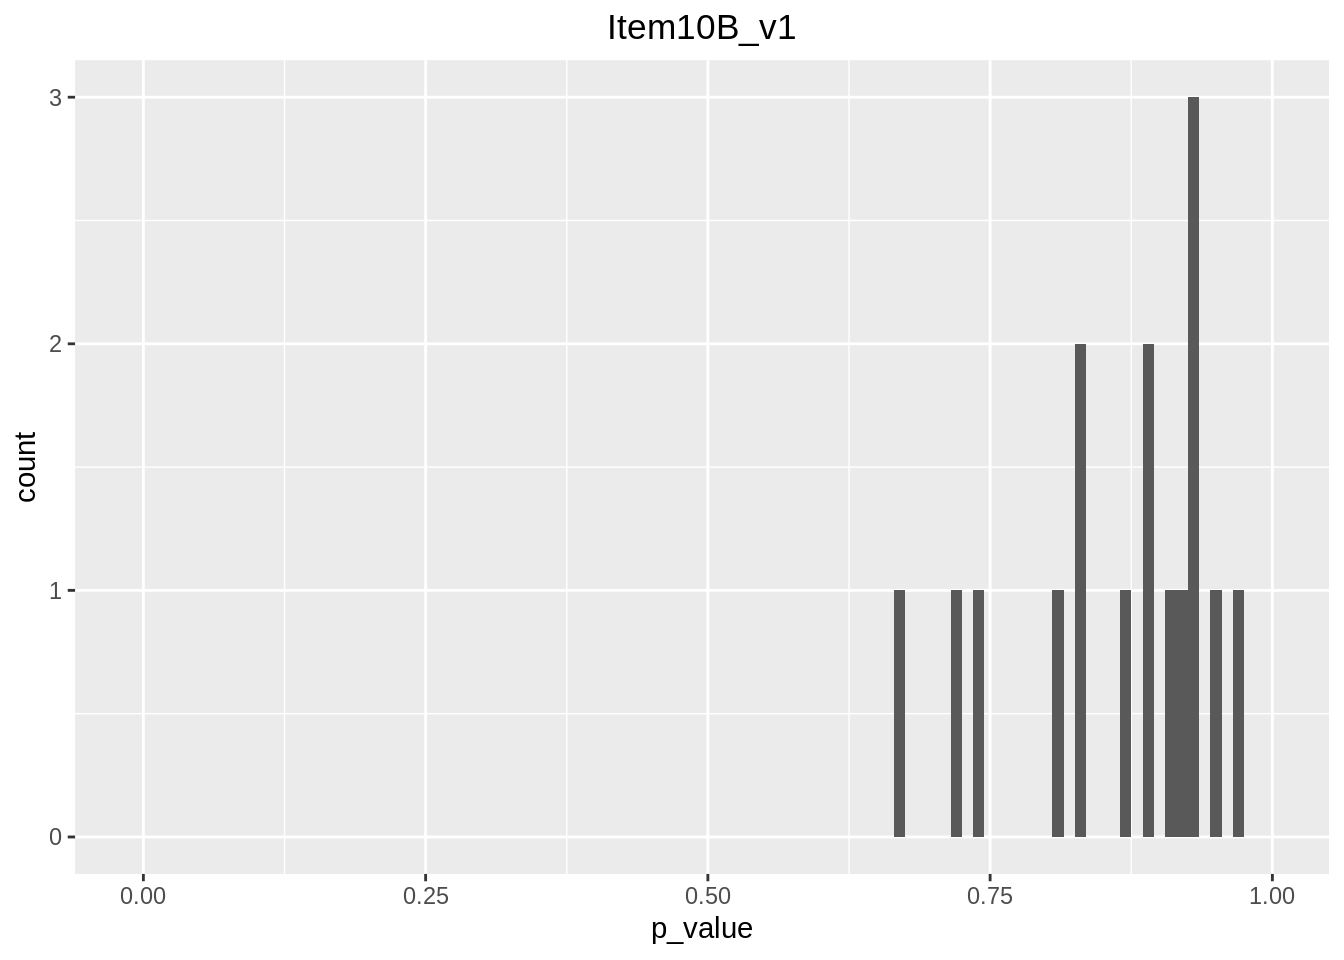
\includegraphics{smartitem_files/figure-latex/unnamed-chunk-9-1.pdf}

\section{Item 14b\_v1}\label{item-14b_v1-1}

\begin{Shaded}
\begin{Highlighting}[]
\NormalTok{fourteenb_v1 =}\StringTok{ }\NormalTok{hp_items_no_cr }\OperatorTok\StringTok{ }\KeywordTok{filter}\NormalTok{(item_id }\OperatorTok{==}\StringTok{ '14B_v1'}\NormalTok{)}
\KeywordTok{kable}\NormalTok{(fourteenb_v1)}
\end{Highlighting}
\end{Shaded}

\begin{tabular}{l|l|r|r}
\hline
item\_id & order\_no\_cr & p\_value & count\\
\hline
14B\_v1 & 0 & 0.4235294 & 170\\
\hline
14B\_v1 & 1 & 0.1511628 & 86\\
\hline
14B\_v1 & 12 & 0.1176471 & 34\\
\hline
14B\_v1 & 123 & 0.1282051 & 39\\
\hline
14B\_v1 & 1234 & 0.4432990 & 97\\
\hline
14B\_v1 & 124 & 0.2903226 & 31\\
\hline
14B\_v1 & 13 & 0.4193548 & 31\\
\hline
14B\_v1 & 134 & 0.4146341 & 41\\
\hline
14B\_v1 & 14 & 0.3333333 & 33\\
\hline
14B\_v1 & 2 & 0.0675676 & 148\\
\hline
14B\_v1 & 23 & 0.2352941 & 51\\
\hline
14B\_v1 & 234 & 0.1562500 & 32\\
\hline
14B\_v1 & 24 & 0.2972973 & 37\\
\hline
14B\_v1 & 3 & 0.2705882 & 85\\
\hline
14B\_v1 & 34 & 0.4255319 & 47\\
\hline
14B\_v1 & 4 & 0.1460674 & 89\\
\hline
\end{tabular}

\subsection{Histogram}\label{histogram-3}

\begin{Shaded}
\begin{Highlighting}[]
\KeywordTok{ggplot}\NormalTok{(fourteenb_v1, }\KeywordTok{aes}\NormalTok{(}\DataTypeTok{x=}\NormalTok{p_value)) }\OperatorTok{+}\StringTok{ }\KeywordTok{geom_histogram}\NormalTok{(}\DataTypeTok{binwidth=}\NormalTok{.}\DecValTok{01}\NormalTok{) }\OperatorTok{+}\StringTok{ }\KeywordTok{labs}\NormalTok{(}\DataTypeTok{title =} \StringTok{"Item14b_v1"}\NormalTok{) }\OperatorTok{+}\StringTok{ }\KeywordTok{xlim}\NormalTok{(}\OperatorTok{-}\NormalTok{.}\DecValTok{01}\NormalTok{,}\DecValTok{1}\NormalTok{)}
\end{Highlighting}
\end{Shaded}

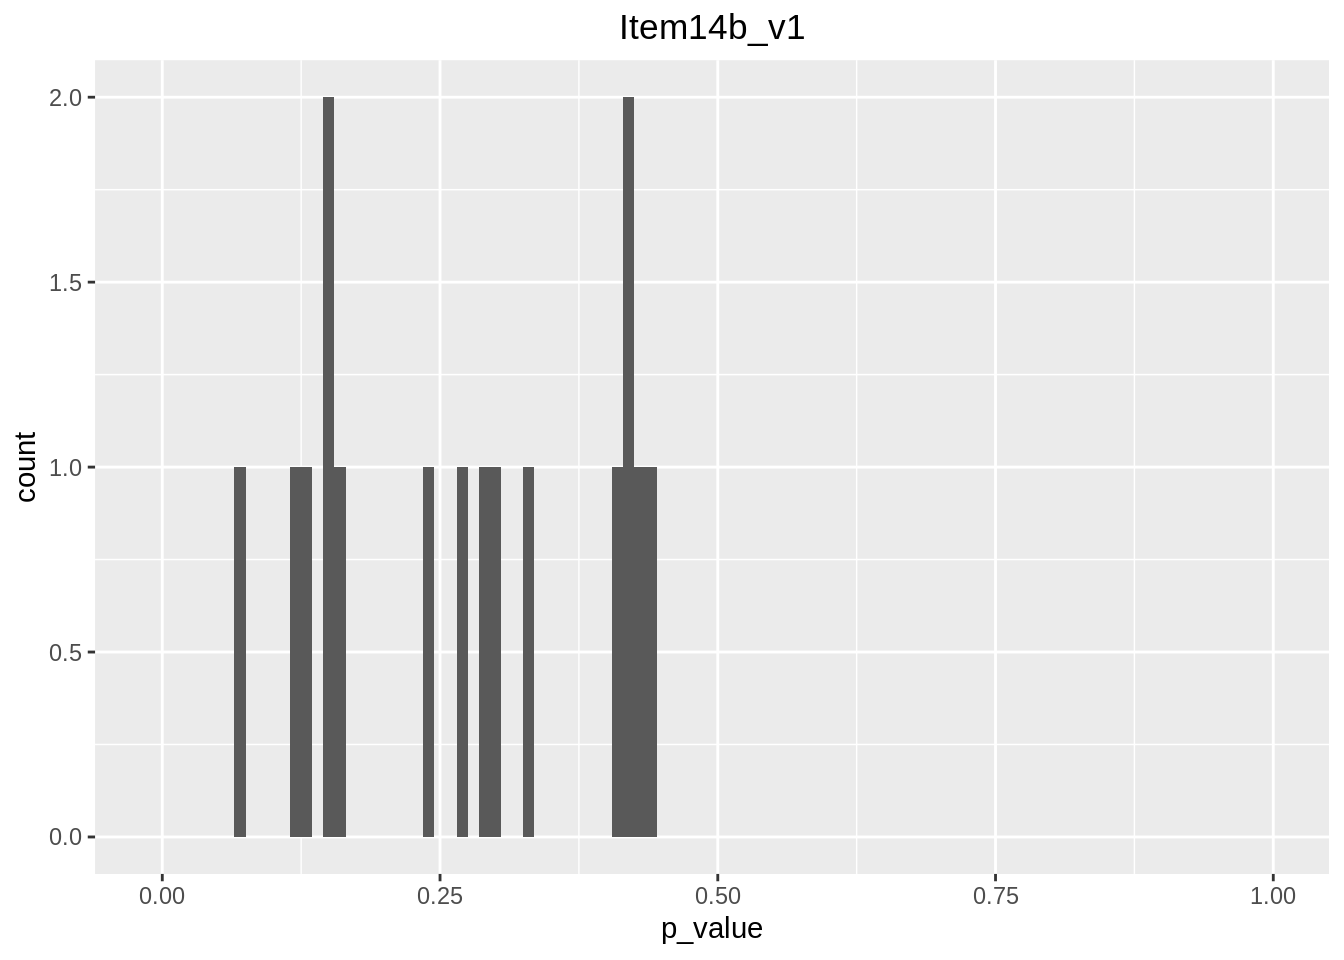
\includegraphics{smartitem_files/figure-latex/unnamed-chunk-11-1.pdf}

\section{All Item Plots}\label{all-item-plots}

\begin{Shaded}
\begin{Highlighting}[]
\NormalTok{knitr}\OperatorTok{::}\NormalTok{opts_chunk}\OperatorTok{$}\KeywordTok{set}\NormalTok{(}\DataTypeTok{fig.width=}\DecValTok{12}\NormalTok{, }\DataTypeTok{fig.height=}\DecValTok{20}\NormalTok{) }

\KeywordTok{ggplot}\NormalTok{(hp_items_no_cr, }\KeywordTok{aes}\NormalTok{(}\DataTypeTok{x=}\NormalTok{p_value)) }\OperatorTok{+}\StringTok{ }\KeywordTok{geom_histogram}\NormalTok{(}\DataTypeTok{binwidth=}\NormalTok{.}\DecValTok{01}\NormalTok{) }\OperatorTok{+}\StringTok{ }\KeywordTok{labs}\NormalTok{(}\DataTypeTok{title =} \StringTok{"All Items"}\NormalTok{) }\OperatorTok{+}\StringTok{ }\KeywordTok{xlim}\NormalTok{(}\OperatorTok{-}\NormalTok{.}\DecValTok{01}\NormalTok{,}\DecValTok{1}\NormalTok{) }\OperatorTok{+}\StringTok{ }\KeywordTok{facet_wrap}\NormalTok{(}\OperatorTok{~}\NormalTok{item_id, }\DataTypeTok{ncol=}\DecValTok{3}\NormalTok{)}
\end{Highlighting}
\end{Shaded}

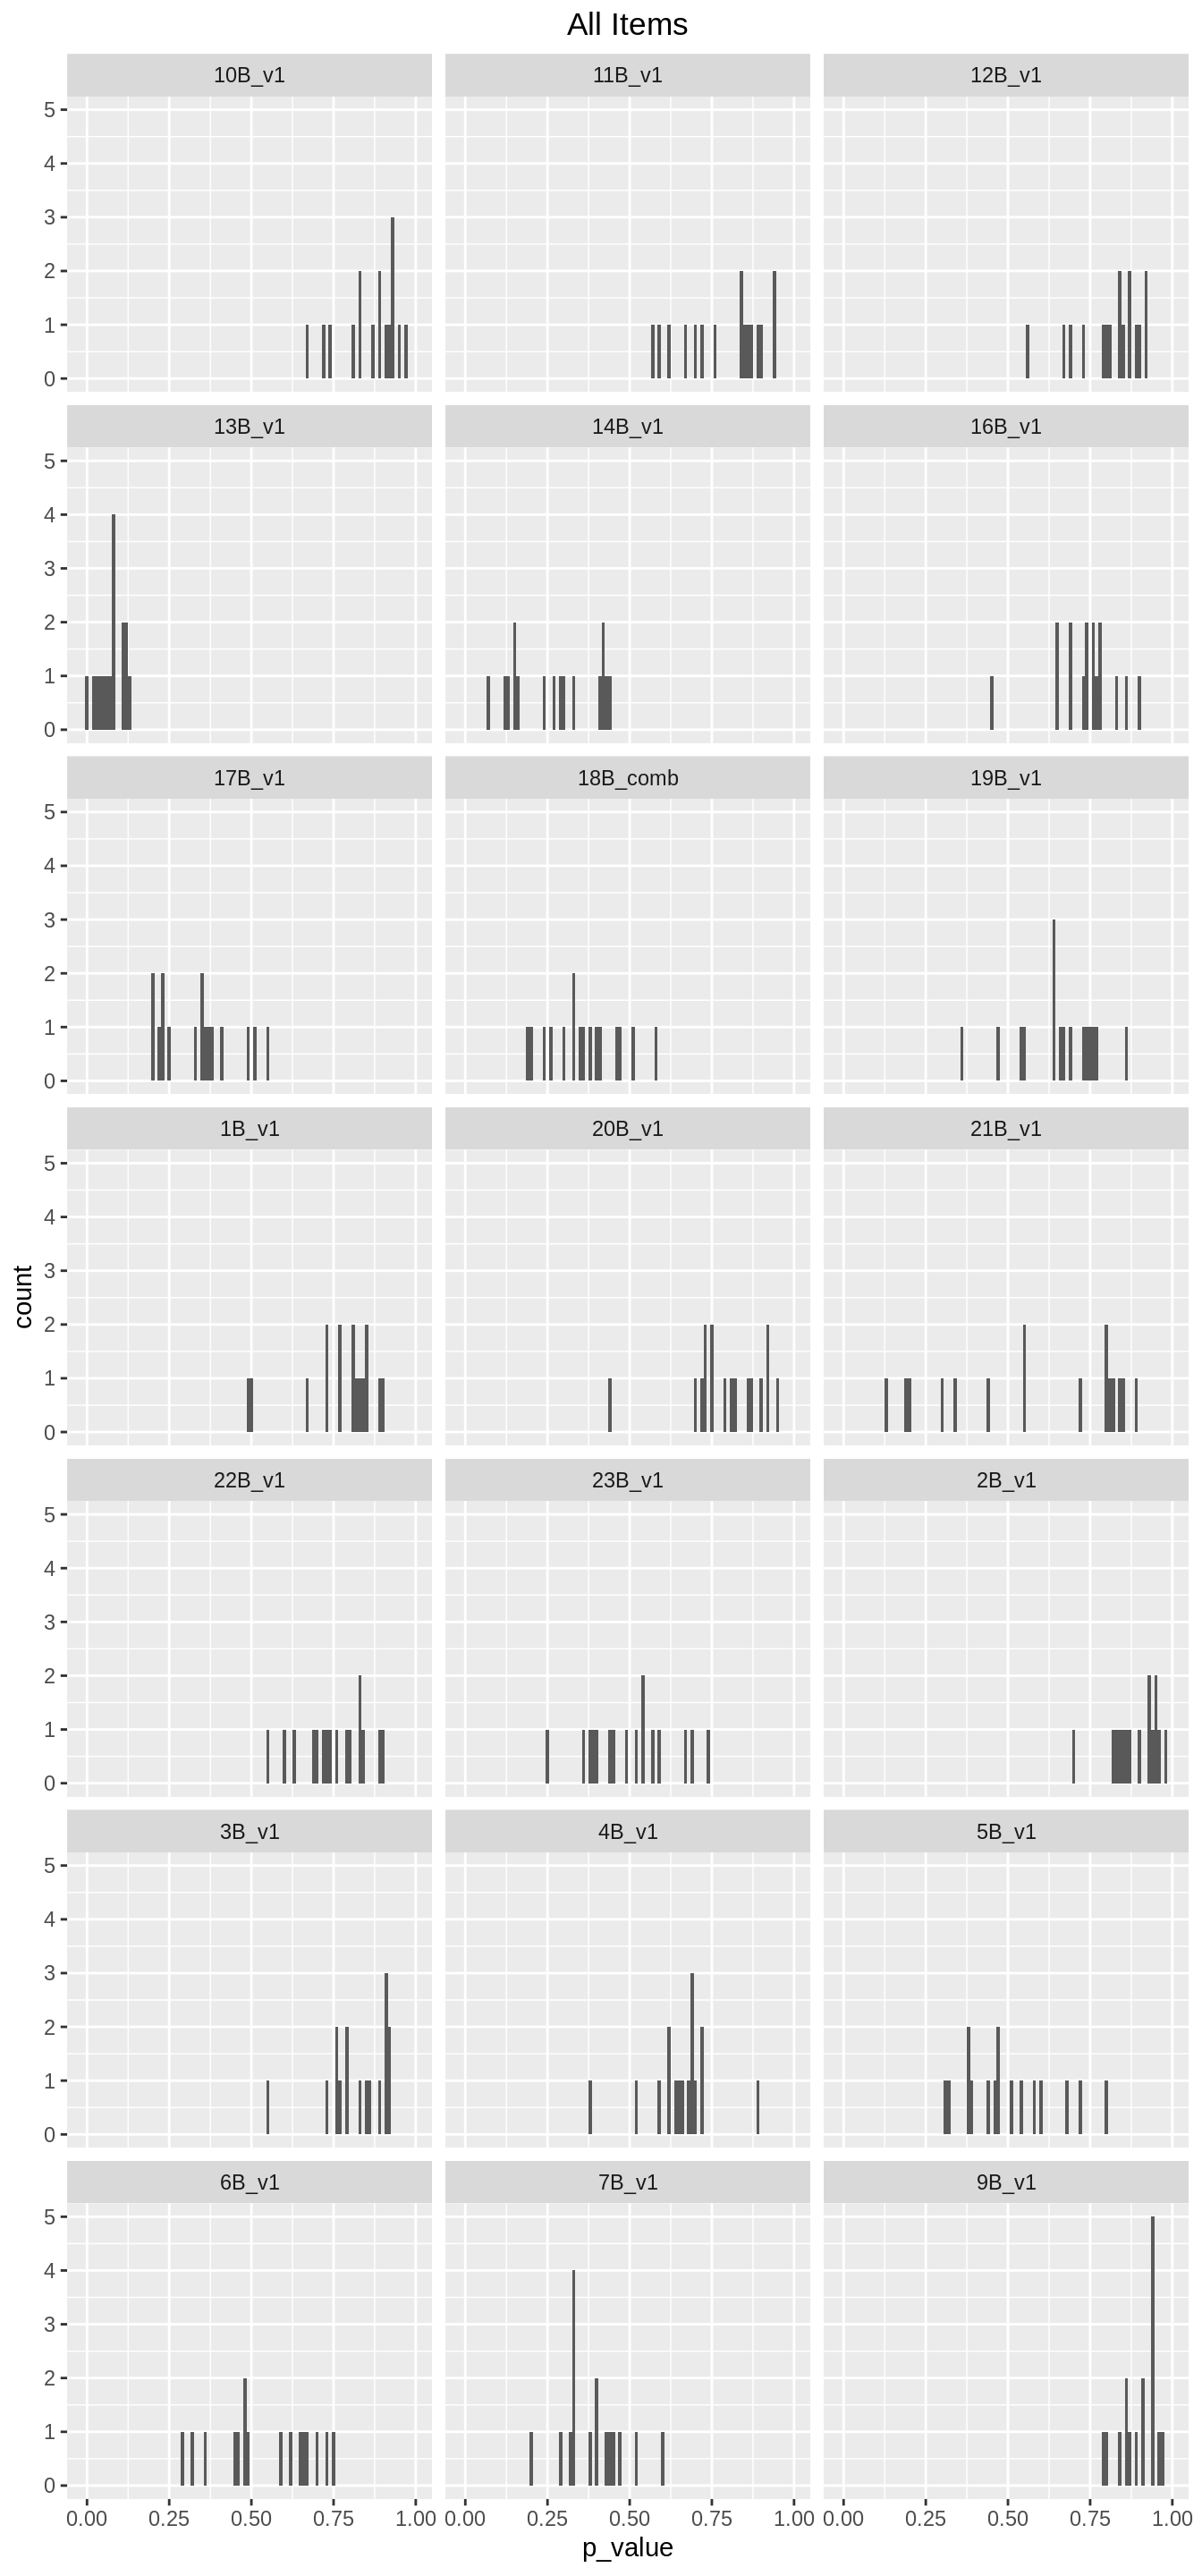
\includegraphics{smartitem_files/figure-latex/unnamed-chunk-12-1.pdf}

\chapter{Final Words}\label{final-words}

We have finished a nice book.

\bibliography{book.bib,packages.bib}


\end{document}
